% vim:autoindent:set textwidth=78:
\section{Comenzando}\label{label_getstarted}

Este capítulo ofrece un vistazo rápido de QGIS funcionando con datos disponibles 
en la página web de QGIS.

\subsection{Instalación}\label{label_installation}
\index{installation}

La compilación de QGIS desde su código fuente está documentada en el Apéndice \ref{sec:install_windows} para Windows, Apéndice \ref{sec:install_macosx} para Mac OSX y Apéndice \ref{sec:install_linux} para GNU/Linux. 
La instrucciones de instalación se distribuyen con el código fuente de QGIS y
también están disponibles en \url{http://qgis.org}. 

Los paquetes estándares de instalación están disponibles para Windows y Mac OS X. 
Se proporcionan los paquetes binarios para la mayoría de sabores de GNU/Linux. 
Obtén la última información sobre los paquetes binarios en el sitio web QGIS
 \url{http://download.qgis.org}.

\subsection{Datos de ejemplo}\label{label_sampledata}
\index{data!sample} 

Si no tienes datos SIG a mano, puedes obtener un conjunto de datos de Alaska
de la web de QGIS \url{http://qgis.org}. La proyección para los datos de Alaska
es Albers Equal Area con las unidades en metros:

\begin{verbatim}
PROJCS["NAD_1927_Albers",
    GEOGCS["GCS_North_American_1927",
	DATUM ["D_North_American_1927",
	     SPHEROID["Clarke_1866", 6378206.4,294.9786982]],
	     PRIMEM["Greenwich",0.0],
	     UNIT["Degree", 0.0174532925199433]],
    PROJECTION["Albers"],
    PARAMETER["False_Easting", 0.0],
    PARAMETER["False_Northing",0.0],
    PARAMETER["Central_Meridian",-154.0],
    PARAMETER["Standard_Parallel_1", 55.0],
    PARAMETER["Standard_Parallel_2",65.0],
    PARAMETER ["Latitude_Of_Origin",50.0],
    UNIT["Meter",1.0]]
\end{verbatim}

Para utilizarlo con GRASS, una base de datos de ejemplo GRASS (p.ej. Spearfish) 
se puede obtener de la web-SIG oficial GRASS \url{http://grass.itc.it/download/data.php}. 
La proyeccción oficial del conjunto de datos de Spearfish es UTM Zone 13, Northern Hemisphere: 

\begin{verbatim}
PROJCS["UTM Zone 13, Northern Hemisphere",
    GEOGCS["clark66",
        DATUM["North_American_Datum_1927",
            SPHEROID["clark66",6378206.4,294.9786982]],
        PRIMEM["Greenwich",0],
        UNIT["degree",0.0174532925199433]],
    PROJECTION["Transverse_Mercator"],
    PARAMETER["latitude_of_origin",0],
    PARAMETER["central_meridian",-105],
    PARAMETER["scale_factor",0.9996],
    PARAMETER["false_easting",500000],
    PARAMETER["false_northing",0],
    UNIT["meter",1]]
\end{verbatim}

Estos conjuntos de datos se utilizarán como base para muchos ejemplos y 
capturas de pantalla en este documento.

\subsection{Iniciando QGIS}\label{label_startinqgis}

Suponiendo que tienes QGIS instalado en el PATH, puedes iniciar QGIS tecleando:
\textbf{qgis}  en línea de comandos o haciendo doble click sobre el enlace a QGIS 
(o acceso directo) sobre el escritorio. Bajo MS Windows, inicia QGIS a través 
del menú Inicio, y bajo Mac OS X, haz doble click en tu carpeta de aplicaciones. 

\subsubsection{Opciones de Línea de Comandos}\index{command line options}
\label{label_commandline}

QGIS soporta un buen número de opciones cuando se inicia desde la línea de 
comandos. Para obtener la lista de opciones, teclea \texttt{qgis ---help} en la
línea de comandos.
La sentencia de uso para QGIS es:

\small
\begin{verbatim}
qgis --help
Quantum GIS - 0.9.0 'Ganymede'
Quantum GIS (QGIS) is a viewer for spatial data sets, including
raster and vector data.
Usage: qgis [options] [FILES]
  options:
        [--snapshot filename]   emit snapshot of loaded datasets to given file
        [--lang language]       use language for interface text
        [--project projectfile] load the given QGIS project
        [--extent xmin,ymin,xmax,ymax]  set initial map extent
        [--help]                this text

  FILES:
    Files specified on the command line can include rasters,
    vectors, and QGIS project files (.qgs):
     1. Rasters - Supported formats include GeoTiff, DEM
        and others supported by GDAL
     2. Vectors - Supported formats include ESRI Shapefiles
        and others supported by OGR and PostgreSQL layers using
        the PostGIS extension
\end{verbatim}
\normalsize

\begin{Tip} \caption{\textsc{Ejemplo utilizando argumentos en línea de comandos}}
\qgistip{Puedes iniciar QGIS especificando uno o más archivos de datos sobre la
línea de comandos. Por ejemplo, suponiendo que estas en tu directorio de datos, 
puedes iniciar QGIS con dos archivos shape y un raster preparados para cargarlos 
con el arranque utilizando el siguiente comando: 
\ttfamily{qgis ak\_shade.tif alaska.shp majrivers.shp}
}
\end{Tip}

\minisec{Opción de línea de comandos \texttt{---snapshot}}
Esta opción te permite crear una captura de pantalla en formato PNG de la vista actual.
Esto puede ser útil cuando tienes muchos proyectos y quieres generar capturas de tus datos.

Actualmente esto genera un fichero PNG con 800x600 pixeles. Se puede añadir un nombre despues de
\texttt{---snapshot}.

\minisec{Opción de línea de comandos \texttt{---lang}}
Basado en tu QGIS local, selecciona la localización correcta. Si quieres cambiar el lenguaje, 
puedes proporcionar otro lenguaje con esta opción.

\minisec{Opción de línea de comandos \texttt{---project}}
También es posible iniciar QGIS con un proyecto existente. Simplemente añade 
la opción \texttt{--project} seguida del nombre de tu proyecto y  QGIS se abrirá 
con todas las capas cargadas definidas en el fichero dado.

\minisec{Opción de línea de comandos \texttt{---extent}}
Para arrancar con un extensión específica del mapa utiliza esta opción. Necesitas
añadir los límites en el siguiente orden separados por comas:
\begin{verbatim}
--extent xmin,ymin,xmax,ymax
\end{verbatim}


\subsection{GUI QGIS (Interfaz Gráfica de Usuario)}\index{main window}
\label{label_qgismainwindow}

Cuando QGIS arranca, te encuentras con la GUI como se muestra abajo
(los números del 1 hasta el 6 en ovalos azules señalan las seis áreas principales 
de la interfaz que se describen abajo):

\begin{figure}[ht]
   \begin{center}
   \caption{Ventana principal con datos de ejemplo de Alaska (GNU/Linux con KDE)}\label{fig:startup}
   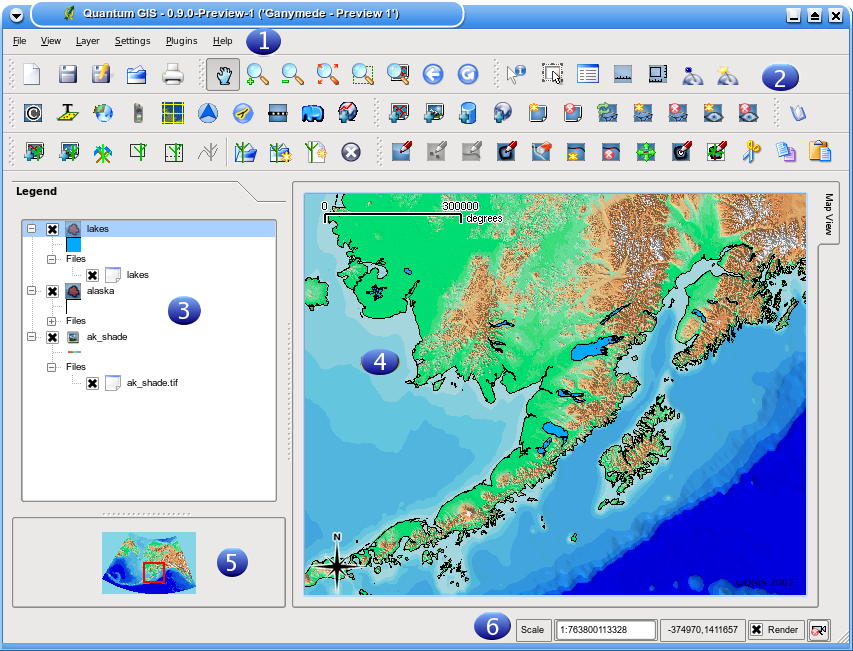
\includegraphics[clip=true, width=17cm]{startup09}
\end{center} 
\end{figure}

\textbf{Nota:} La decoración de tu ventana (barra de título, etc.) puede aparecer 
distinto dependiendo de tu sistema operativo y administrador de ventanas.

La Interfaz Gráfica de Usuario (GUI) de QGIS está dividida en seis áreas:

\begin{tabbing}
1. Barra de Menús \hspace{3cm}\= 4. Vista de Mapa \\
2. Barra de Herramientas \hspace{3cm}\> 5. Vista General  \\
3. Leyenda del Mapa \hspace{3cm}\> 6. Barra de Estado   
\end{tabbing}

Estos seis componentes de la interfaz de QGIS están descritos con más detalle
en las siguientes secciones.

\subsubsection{Barra de Menús}\label{label_menubar}
\index{menus}

La barra de menús proporciona acceso a varias características de QGIS utilizando 
menús jerárquicos estándares. El nivel superior de los menús y un extracto de 
algunas funciones proporcionadas son:

\begin{itemize}

\item \textbf{Archivo}
\begin{itemize}
\item \textbf{Proyecto Nuevo}          - ver Sección \ref{sec:projects}
\item \textbf{Abrir Proyecto}         - ver Sección \ref{sec:projects}
\item \textbf{Abrir Proyectos recientes} - ver Sección \ref{sec:projects}
\item \textbf{Guardar Proyecto}         - ver Sección \ref{sec:projects}
\item \textbf{Guardar Proyecto Como}      - ver Sección \ref{sec:projects}
\item Guardar como imágen
\item Exportar a Mapa de MapServer       - ver Sección \ref{sec:mapserver_export}
\item Imprimir                         - ver Sección \ref{label_mapcomposer}
\item Salir
\end{itemize}

\item \textbf{Ver}
\begin{itemize}
\item Zoom General
\item Zoom a Selección
\item Zoom a Capa
\item Zoom Anterior
\item Refrescar
\item Mostrar Marcadores
\item Nuevo Marcador
\item Mostrar todas las Barras de Herramientas posibles
\item Ocultar todas las Barras de Herramientas posibles
\item Visibilidad de Barra de Herramientas 
\end{itemize}

\item \textbf{Capa}
\begin{itemize}
\item \textbf{Añadir una Capa Vectorial}       - ver Sección \ref{label_workingvector}
\item \textbf{Añadir una Capa Raster}       - ver Sección \ref{label_raster}
\item \textbf{Añadir una Capa PostGIS}      - ver Sección \ref{label_postgis}
\item \textbf{Añadir una Capa WMS}          - ver Sección \ref{sec:ogc-wms}
\item Eliminar Capa
\item Nueva Capa Vectorial          	- ver Sección \ref{sec:create shape}
\item Llevar al Localizador
\item Añadir Todo al Localizador
\item Eliminar Todo del Localizador
\item Ocultar todas las Capas
\item Mostrar todas las Capas
\end{itemize}

\item \textbf{Configuración}
\begin{itemize}
\item \textbf{Propiedades del Proyecto}  - ver Sección \ref{sec:projects}
\item \textbf{Proyección Personalizada}   - ver Sección \ref{sec:customprojections}
\item \textbf{Opciones}             - ver Sección \ref{subsec:gui_options}
\end{itemize}

\item \textbf{Complementos} - (Posteriores elementos del menú serán añadidos por los complementos según se vayan añadiendo.)
\begin{itemize}
\item Administrador Complementos          	   - ver Sección \ref{sec:managing_plugins}
\end{itemize}          	

\item \textbf{Ayuda}
\begin{itemize}
\item Contenido de la Ayuda
\item Página web de QGIS
\item Comprobar Versión de QGIS 
\item Acerca de
\end{itemize}

\end{itemize}

%See Appendix \ref{app_menu} for complete descriptions of the menu items.

\subsubsection{Barras de Herramientas}\label{label_toolbars}
\index{toolbars}

The toolbars provide access to most of the same functions as the menus,
plus additional tools for interacting with the map. Each toolbar item has
popup help available. Hold your mouse over the item and a short description of
the tool's purpose will be displayed. 

Every menubar can be moved around according to your needs. Additionally every
menubar can be switched off using your right mouse button context menu holding
the mouse over the toolbars.

\begin{Tip}
\caption{\textsc{Reappearing toolbars}} \index{layout!toolbars}
\qgistip{If you have accidentally hidden all your toolbars, you can get them back by
choosing \texttt{Show most toolbars} from the View|Toolbars menu.}
\end{Tip}

\subsubsection{Map Legend}\label{label_legend}
\index{legend}

% TODO The new legend features need to be described here briefly.
% Marco, would you make a start what is new in the legend?!
The map legend area is used to set the visibility and z-ordering of layers.
Z-ordering means that layers listed nearer the top of the legend are drawn
over layers listed lower down in the legend. The checkbox in each legend
entry can be used to show or hide the layer.\index{layer!visibility}

Layers can be grouped in the legend window by adding a layer group and dragging layers 
into the group. To do so, go with the mouse to the legend window, right click, choose 'Add group'. 
A new folder appears. Now drag the layers to the folder symbol. It is then possible to toggle the 
visibility of all the layers in the group with one click. To bring layers out of a group, go with 
the mouse to the layer symbol, right click, choose 'Make to toplevel item'. To give the folder a 
new name, choose 'Rename' in the right click menu of the group.

The content of the right mouse button context menu depends on if the loaded legend item you hold your 
mouse over is a raster or a vector layer. For GRASS vector layers the 'toggle editing' is not 
available. See section \ref{grass_digitising} for infos on editing GRASS vector layers. 

\begin{itemize}

\item \textbf{Right mouse button menue for raster layers}
\begin{itemize}
\item Zoom to layer extend
\item Zoom to best scale (100\%)
\item Show in overview
\item Remove
\item Properties
\item Rename
\item Add Group
\item Expand all
\item Collapse all
\item Show file groups
\end{itemize}

\item \textbf{Right mouse button menue for vector layers}
\begin{itemize}
\item Zoom to layer extend
\item Show in overview
\item Remove
\item Open attribute table
\item Toggle editing (not available for GRASS layers)
\item Save as shapefile
\item Save selection as shapefile
\item Properties
\item Rename
\item Add Group
\item Expand all
\item Collapse all
\item Show file groups
\end{itemize}

\item \textbf{Right mouse button menue for layer groups} 
\begin{itemize}
\item Remove
\item Rename
\item Add Group
\item Expand all
\item Collapse all
\item Show file groups
\end{itemize}

\end{itemize}

If several vector data sources have the same vector type and the same attributes, their 
symbolisations may be grouped. This means that if the symbolisation of one data source is 
changed, the others automatically have the new symbolisation as well. To group symbologies, open 
the right click menu in the legend window and choose 'Show file groups'. The file groups of the 
layers appear. It is now possible to drag a file from one file group into another one. If this is done, 
the symbologies are grouped. Note that QGIS only permits the drag if the two layers are able to share 
symbology (same vector type and same attributes).  

%% isn't included in Titan anymore, except for an "toggle overview"
%Each legend entry can show the following mini icons:
%
%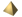
\includegraphics[width=0.7cm]{pyramid} This is a raster
%that has pyramids built for it to improve rendering efficiency (see
%Section \ref{raster_pyramids}).\\
%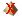
\includegraphics[width=0.7cm]{no_pyramid} This is a
%raster that has no pyramid layers (see Section \ref{raster_pyramids}).\\
%
\includegraphics[width=0.7cm]{inoverview} This layer is
%shown in the overview map area as well as in the main map window.\\
%
\includegraphics[width=0.7cm]{editable} This is a vector
%layer that is currently enabled for editing.\\

\subsubsection{Map View}\label{label_mapview}
\index{map!view}

This is the 'business end' of QGIS - maps are displayed in this area! The
map displayed in this window will depend on the vector and raster layers you
have chosen to load (see sections that follow for more information on how to
load layers). The map view can be panned (shifting the focus of the map display
to another region) and zoomed in and out. Various other operations can be
performed on the map as described in the toolbar description above.  The map
view and the legend are tightly bound to each other - the maps in view reflect
changes you make in the legend area.  

\begin{Tip}\caption{\textsc{Zooming the Map with the Mouse
Wheel}}\index{zoom!mouse wheel}
\qgistip{You can use the mouse wheel to zoom in and out on the map. Place
the mouse cursor inside the map area and roll it forward (away from you) to
zoom in and backwards (towards you) to zoom out. The mouse cursor is the 
center where the zoom occurs. You can customize the behavior of the mouse
wheel zoom using the \texttt{Map tools} tab under the Settings|Options menu.  }
\end{Tip}

\subsubsection{Map Overview}\label{label_mapoverview}
\index{map!overview}

The map overview area provides a full extent view of layers added to it.
Within the view is a rectangle showing the current map extent. This allows
you to quickly determine which area of the map you are currently viewing. Note
that labels are not rendered to the map overview even if the layers in the
map overview have been set up for labeling. 
You can add a single layer to the
overview by right-clicking on it in the legend and choosing \textit{Add
to overview}. You can also add or remove all layers to the overview using the
Overview tools on the toolbar.

You can also grab the red rectangle showing your current extent and pan around; the
map view will update accordingly.

\subsubsection{Status Bar}\label{label_statusbar}

The status bar shows you your current position in map coordinates (e.g.
meters or decimal degrees) as the mouse pointer is moved across the map view.
The status bar also shows the view extents of the map view as you pan and
zoom in and out. A progress bar in the status bar shows progress of rendering
as each layer is drawn to the map view. In some cases, such as the gathering
of statistics in raster layers, the progress bar will be used to show the
status of lengthy operations. On the right side of the status bar is a small
checkbox which can be used to temporarily prevent layers being rendered to the
map view (see Section \ref{subsec:redraw_events} below). At the far right of
the status bar is a projector icon. Clicking on this opens the projection
properties for the current project.

\subsection{Rendering}\label{subsec:redraw_events}\index{rendering}

By default, QGIS renders all visible layers whenever the map canvas must be
refreshed. The events that trigger a refresh of the map canvas include:

\begin{itemize}
\item Adding a layer
\item Panning or zooming
\item Resizing the QGIS window
\item Changing the visibility of a layer or layers
\end{itemize}

QGIS allows you to control the rendering process in a number of ways.

\subsubsection{Scale Dependent Rendering}\index{rendering!scale dependent}
\label{label_scaledepend}

Scale dependent rendering allows you to specify the minimum and maximum
scales at which a layer will be visible.  To set scale dependency rendering,
open the properties dialog by double-clicking on the layer in the legend. On
the \textit{General} tab, set the minimum and maximum scale values and then
click on the \textit{Use scale dependent rendering} checkbox.

You can determine the scale values by first zooming to the level you want
to use and noting the scale value in the QGIS status bar.\index{scale}

\subsubsection{Controlling Map Rendering}\label{label_controlmap}

Map rendering can be controlled in the following ways:

\minisec{Suspending Rendering}\index{rendering!suspending}
\label{label_suspendrender}

To suspend rendering, click the \textit{Render} checkbox in the lower right
corner of the statusbar. When the \textit{Render} box is not checked, QGIS
does not redraw the canvas in response to any of the events described in
Section \ref{subsec:redraw_events}. Examples of when you might want to suspend
rendering include:

\begin{itemize}
\item Add many layers and symbolize them prior to drawing
\item Add one or more large layers and set scale dependency before drawing
\item Add one or more large layers and zoom to a specific view before
drawing
\item Any combination of the above
\end{itemize}

Checking the \textit{Render} box enables rendering and causes and immediate
refresh of the map canvas.

\minisec{Setting Layer Add Option}\label{label_settinglayer}
\index{rendering!options}\index{layers!initial visibility}

You can set an option to always load new layers without drawing them. This
means the layer will be added to the map, but its visibility checkbox in the
legend will be unchecked by default. To set this option, choose
\textit{Options} from the \textit{Settings} menu and click on the
\textit{Rendering} tab. Check the \textit{New layers added to the map are not
displayed} checkbox. Any layer added to the map will be off (invisible) by
default.

%\minisec{Stopping Rendering}\index{rendering!halting}
%\label{label_stoprender}
%
%To stop the map drawing, press the ESC key. This will halt the refresh of
%the map canvas and leave the map partially drawn. It may take a bit of time
%between pressing ESC and the time the map drawing is halted.
%
%\textbf{NOTE}: It is currently not possible to stop rendering - this was disabled 
%in qt4 port because of User Interface (UI) problems and crashes.

\minisec{Updating the Map Display During Rendering}
\label{label_updatemap}\index{rendering!update during drawing}

You can set an option to update the map display as features are drawn. By
default, QGIS does not display any features for a layer until the entire
layer has been rendered. To update the display as features are read from the
datastore, choose \textit{Options} from the \textit{Settings} menu and
click on the \textit{Rendering} tab. Set the feature count to an
appropriate value to update the display during rendering. Setting a value of 0
disables update during drawing (this is the default). Setting a value too low
will result in poor performance as the map canvas is continually updated
during the reading of the features. A suggested value to start with is 500. 

\subsection{Measuring}\label{sec:measure}\index{measure}

Measuring works within projected coordinate systems only (e.g., UTM). If 
the loaded map is defined with a geographic coordinate system
(latitude/longitude), the results from line or area measurements will be 
incorrect. To fix this you need to set an appropriate map coordinate system.

\subsubsection{Measure length}\index{measure:line length}

\includegraphics[width=0.7cm]{measureline} QGIS is also able to measure real distances between given 
points according to a defined ellipsoid. Therefore choose \textit{Options} from the \textit{Settings} menu, 
click on the \textit{Map tools} tab and choose the appropriate ellipsoid. The tool then allows you to 
click points on the map. Each segment-length shows up in the measure-window and additionaly the total 
length is printed. To stop measuring click your right mouse button. 

\subsubsection{Measure areas}\index{measure:areas}

\includegraphics[width=0.7cm]{measurearea} Also areas can be measured. The window only shows the
accumulated area-size in the measure window (see figure \ref{fig:measure}).

% measure-tools side by side
\begin{figure}[h]
\caption{Measure tools in action} \label{fig:measure}
\centering
   \subfigure[Measure lines] {\label{subfig:measure_line}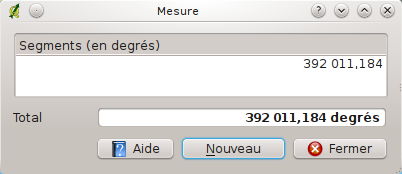
\includegraphics[clip=true, width=0.4\textwidth]{measure_line}}\goodgap
   \subfigure[Measure areas]{\label{subfig:measure_area}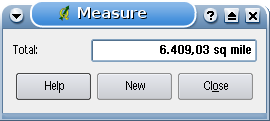
\includegraphics[clip=true, width=0.4\textwidth]{measure_area}}
\end{figure}

\subsection{Projects}\label{sec:projects}\index{projects}

The state of your QGIS session is considered a Project.  QGIS
works on one project at a time.  Settings are either considered
as being per-project, or as a default for new projects (see
Section \ref{subsec:gui_options}).

QGIS can save the state of your workspace into a project file using
the menu option \textit{File}->\textit{Save Project}.

Loading saved projects is a similar process.

The kinds of information saved in a project file include:

\begin{itemize}
\item Layers added
\item Layer properties, including symbolization
\item Projection for the map view
\item Last viewed extent
\end{itemize}

The project file is saved in XML format, so it is possible to edit
the file outside QGIS if you know what you are doing.  

The file format was updated several times compared to earlier QGIS versions. Project files 
from older QGIS versions may not work properly anymore.

\subsection{GUI Options}
\label{subsec:gui_options}

\includegraphics[width=0.7cm,clip=true]{options} Some basic options for QGIS
can be selected using the Options dialog. Select the \textsl{Settings} entry
from the menu and choose \textsl{Options} (Alt-O). The tabs where you can 
optmize your options are:

\minisec{General Tab}

\begin{itemize}
\item ask to save project changes when required
\end{itemize}

\minisec{Appearance Tab}

\begin{itemize}
\item Hide or show splash screen at startup
\item Change the icon theme 
\item Change Selection and backgroud Color
\item Make layer names appear with Capitals
\end{itemize}

\minisec{Rendering Tab}

\begin{itemize}
\item Update features during drawing or not until all features have been read.
\item Set new layer visible or unvisible when loaded 
\item Make lines appear less jagged at the expense of some drawing performance
\item Fix problems with incorrectly filled polygons
\item Continously redraw when dragging the legend/map divider 
\end{itemize}

\minisec{Map tools Tab}

\begin{itemize}
\item Define Search Radius as a percentage of the map width
\item Define Ellipsoid for distance calculations
\item Set Rubberband Color for Measure Tool
\item Define Mouse wheel action (Zoom, Zoom and recenter, Nothing)
\item Set Zoom factor for wheel mouse
\end{itemize}

\minisec{Projection Tab}

\begin{itemize}
\item Define what to do, when a layer is loaded without projection information
\begin{itemize}
\item Prompt for projection
\item Project wide default projection will be used
\item Global default projection displayed below will be used
\end{itemize}
\end{itemize}

\minisec{Locale Tab}

\begin{itemize}
\item Overwrite system locale and use defined locale instead
\item Information about active system locale
\end{itemize}

\minisec{Help Browser Tab}

\begin{itemize}
\item Define Browser to display help documents
\end{itemize}

You can modify the options according to your needs. Some of the changes may 
require a restart of QGIS before they will be effective.

On GNU/Linux everything is saved in:
\begin{verbatim}
$HOME/.config/QuantumGIS/qgis.conf
\end{verbatim}
This is a normal text file consisting of blocks, where QGIS saves its current
display options, PostGIS and WMS connections, and other settings.

On Windows settings are stored in the registry under:
\begin{verbatim}
\\HKEY_CURRENT_USER\Software\QuantumGIS\qgis
\end{verbatim}

On OS X you can find your settings in:
\begin{verbatim}
$HOME/Library/Preferences/org.qgis.qgis.plist
\end{verbatim}


\subsection{Spatial Bookmarks}\label{sec:bookmarks}
\index{bookmarks}
\index{spatial bookmarks|\see{bookmarks}}

Spatial Bookmarks allow you to ``bookmark'' a geographic location and return to it later.

\subsubsection{Creating a Bookmark}
To create a bookmark:
\begin{enumerate}
\item Zoom or pan to the area of interest.
\item Select the menu option \textit{View}->\textit{New Bookmark} or type Ctrl-B.
\item Enter a descriptive name for the bookmark (up to 255 characters).
\item Click \textit{OK} to add the bookmark or \textit{Cancel} to exit without adding the bookmark.
\end{enumerate}

Note that you can have multiple bookmarks with the same name.

\subsubsection{Working with Bookmarks}
To use or manage bookmarks, select the menu option \textit{View}->\textit{Show Bookmarks}.
The bookmarks dialog allows you to zoom to or delete a bookmark.
You can not edit the bookmark name or coordinates.

\subsubsection{Zooming to a Bookmark}
From the Bookmarks dialog, select the desired bookmark by clicking on it, 
then click the \textit{Zoom To} button.
You can also zoom to a bookmark by double-clicking on it.

\subsubsection{Deleting a Bookmark}
To delete a bookmark from the Bookmarks dialog, click on it then click the \textit{Delete} button.
Confirm your choice by clicking \textit{Yes} or cancel the delete by clicking \textit{No}.
